\documentclass[12pt, letterpaper]{article}
\usepackage{geometry}
\usepackage[utf8]{inputenc}
\usepackage[english]{babel}
\usepackage[runin]{abstract}
\usepackage{titling}
\usepackage{booktabs}
\usepackage{mathtools}
\usepackage{fancyhdr}
\usepackage{helvet}
\usepackage{hyperref}
\usepackage{csquotes}
\usepackage{pgfplots}
\usepackage{graphicx}
\usepackage{blindtext}
\usepackage{tabularx}
\usepackage{parskip}
\usepackage{etoolbox}
\usepackage{amsmath}
\usepackage{amssymb}
\usepackage{multicol}
\usepackage{xcolor}
\usepackage{comma}
\usepackage{wrapfig}
\usepackage{array} % for adjusting padding
\usepackage[makeroom]{cancel}

\usepackage{cellspace} % for controlling vertical padding in cells
\setlength\cellspacetoplimit{6pt} % adjust top padding
\setlength\cellspacebottomlimit{6pt} % adjust bottom padding

\input{preamble.tex}

\title{\textbf{Science: UAM Equations and Projectile Motion Reviewer}}
\runningtitle{UAM Equations}
\author{Lance Dy Chua}
\runningauthor{Lance Dy Chua}
\affiliation{Xavier School San Juan}
\memoid{Lance's Handout}
\theyear{2024}
\mydate{\today}
\graphicspath{{}}
\usepgfplotslibrary{external}
\tikzexternalize

\begin{document}

\maketitle
\graphicspath{ {./Graphs} }

\noindent\section{Format of this Reviewer}

\noindent This reviewer will contain each formula its purpose and some examples. Right now, it doesn't contain much information but I will continue to add details as the days pass. Also take note of the variables; some other resources use different letters to signify values. For example, displacement is often used as $s$ in most resources but can also be used as $\Vec{d}$ or sometimes even $\Delta x$ in math classes. Sometimes initial velocity and final velocity is denoted by $v$ and $u$ respectively. This reviewer was made in pure LaTeX, here is the GitHub if you want it for some reason: 

\noindent\section{Uniformly Accelerated Motion Equations}

\noindent Uniformly accelerated motion equations are essential in physics to describe the motion of an object under constant acceleration. Here are the fundamental equations:

\newcolumntype{Y}{>{\centering\arraybackslash}X} % Adjust as per your requirement

\begin{center}
    \setlength{\tabcolsep}{10pt} % Adjust horizontal padding
    \renewcommand{\arraystretch}{1.5} % Adjust vertical padding

    \begin{tabularx}{\textwidth} { 
        | >{\raggedright\arraybackslash}Y 
        | >{\raggedright\arraybackslash}Y 
        | >{\raggedright\arraybackslash}Y | }
    \hline
    $v_i$ = initial velocity & $v_f$ = final velocity & $d$ = distance\\
    $a$ = acceleration & $t$ = time & $s$ or $\Delta x$ = displacement\\
    \hline
    \end{tabularx}

    \bigskip

    \begin{tabularx}{\textwidth} { 
        | >{\raggedright\arraybackslash}Y 
        | >{\raggedright\arraybackslash}Y 
        | >{\raggedright\arraybackslash}Y | }
    \hline
    ($s$): $v_f = v_i + at$ & ($t$): $v_f^2 = v_i^2 + 2as$ & $ $\\
    ($v_f$): $s = v_i t + \frac{1}{2} at^2$ & ($a$): $s = \frac{1}{2}(v_i + v_f)t$ & ($v_i$): $s = v_f t - \frac{1}{2} at^2$\\
    \hline
    \end{tabularx}
\end{center}

\newpage

\noindent\section{Free Falling}

\newcounter{boxlblcounter}  
\newcommand{\makeboxlabel}[1]{\fbox{#1.}\hfill}% \hfill fills the label box
\newenvironment{boxlabel}
  {\begin{list}
    {\arabic{boxlblcounter}}
    {\usecounter{boxlblcounter}
     \setlength{\labelwidth}{3em}
     \setlength{\labelsep}{0em}
     \setlength{\itemsep}{2pt}
     \setlength{\leftmargin}{1.5cm}
     \setlength{\rightmargin}{2cm}
     \setlength{\itemindent}{0em} 
     \let\makelabel=\makeboxlabel
    }
  }
{\end{list}}

\noindent A free falling problem has a few notable properties:

\setlength{\columnsep}{1cm}
\setlength{\columnseprule}{0.2pt}
\begin{multicols}{2}
    \begin{boxlabel}
        \item No air resistance is taken into account
        \item No external forces aside from gravity
        \item The accelerating force is gravity
        \item The path formed is a parabola
    \end{boxlabel}

    \noindent\centering Also has time symmetry
    
    \includegraphics[width=\textwidth / 4]{Graphs/symmetry.png}
\end{multicols}

\newpage
\noindent\section{Projectile Motion}

\noindent Projectile Motion combines the two concepts we talked about earlier, Horizontal and Vertical motion. Combining these two, you get the following properties

\begin{boxlabel}
    \item No air resistance is taken into account
    \item Assume a perfectly flat planet (no curvature and exit velocity)
    \item The only accelerating force is G (gravity)
    \item The path formed is a parabola, which is symmetric in time
    \item Here's a link to a Desmos live simulation of what the projectile path would look like: https://www.desmos.com/calculator/pcnyhs0n3o
    \includegraphics[width=\textwidth * \real{0.9}]{Graphs/desmos-example1.png}
\end{boxlabel}

\newpage
\noindent As of now, there are only 2 types of Projectile Motion:

\begin{boxlabel}
    \item Type 1: Only has horizontal initial velocity. Since all Type 1 Projectiles having zero vertical initial velocity, in a super ideal flat world with no air resistance, all Type 1 Projectiles dropped at the same height will hit the ground at the same time. If I threw a ball horizontally in a vacuum, it would land at the same exact time as if I just had dropped it. In a Type 1 Projectile, the projectile is not thrown upwards or downwards, only.
    \item Type 2: Has a vector as an initial velocity. This initial velocity is denoted by $\vec{v_i}$ which is a vector. If we wanted it to have a horizontal velocity of $5m/s^2$, we might write it as $\vec{v_i}=\begin{bmatrix}
        5\\5
    \end{bmatrix}$ or as $v_{ix}=5$ and $v_{iy}=5$.
    \item Both Type 1 and Type 2 Projectiles are parabolic. This means that the velocity of the ball is equal to $-9.81x$, and its actual height goes down at a rate of $-9.81x^2$ where $x$ is time.
\end{boxlabel}
\newpage

\noindent Here is a plot of what an object looks like as it is falling from 800 meters in the sky without air resistance. Notice how it starts so slowly, but speeds up very quickly. This is because the velocity changes linearly, which makes the position change exponentially, at a rate of $-9.81t^2$, where $t$ is the time.\\

\begin{center}
    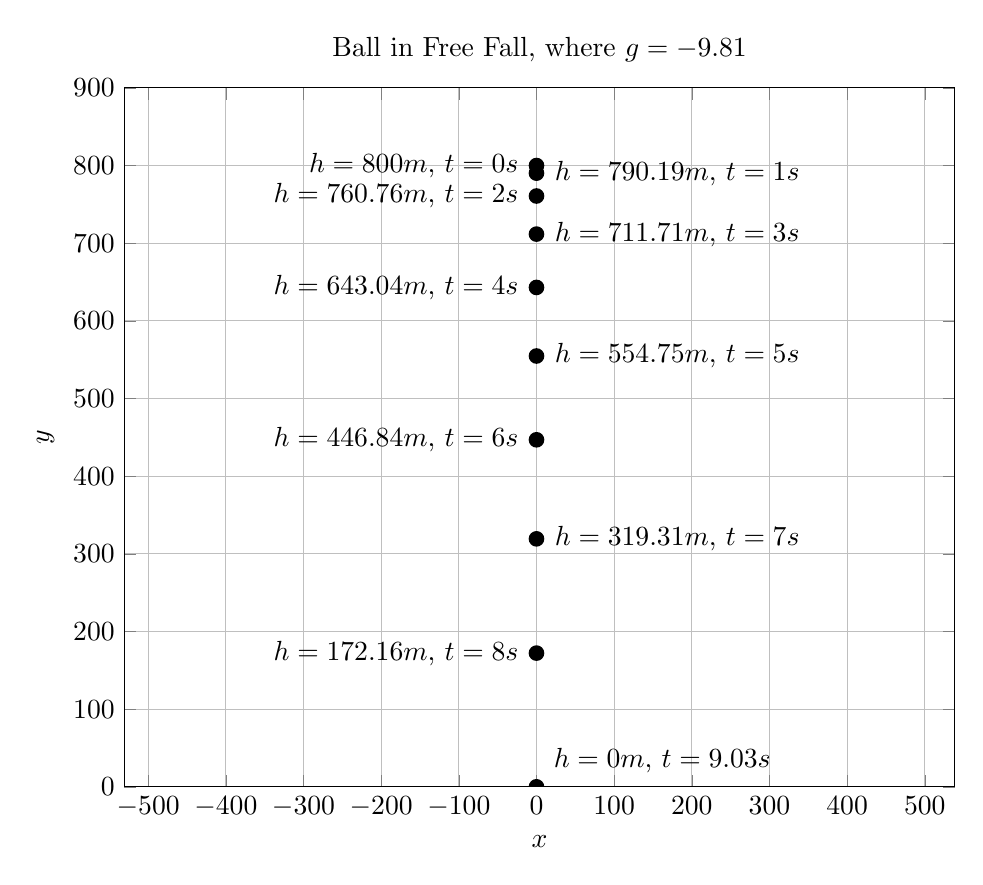
\begin{tikzpicture}
        \begin{axis}[
            title={Ball in Free Fall, where $g=-9.81$},
            axis equal,
            xlabel={$x$},
            ylabel={$y$},
            grid=major,
            legend pos=north west,
            width=\textwidth,
            xmin=0, xmax=8,
            ymin=0, ymax=900,
            legend style={nodes={scale=1, transform shape}}, 
            ]
            % Vector from origin to (1/sqrt(2), 1/sqrt(2))
            \node[label={180:{$h=800m$, $t=0s$}},circle,fill,inner sep=2pt] at (axis cs:0,800) {};
            \node[label={[label distance=0.01em]0:{$h=790.19m$, $t=1s$}},circle,fill,inner sep=2pt] at (axis cs:0,790.19) {};
            \node[label={180:{$h=760.76m$, $t=2s$}},circle,fill,inner sep=2pt] at (axis cs:0,760.76) {};
            \node[label={[label distance=0.01em]0:{$h=711.71m$, $t=3s$}},circle,fill,inner sep=2pt] at (axis cs:0,711.71) {};
            \node[label={180:{$h=643.04m$, $t=4s$}},circle,fill,inner sep=2pt] at (axis cs:0,643.04) {};
            \node[label={[label distance=0.01em]0:{$h=554.75m$, $t=5s$}},circle,fill,inner sep=2pt] at (axis cs:0,554.75) {};
            \node[label={180:{$h=446.84m$, $t=6s$}},circle,fill,inner sep=2pt] at (axis cs:0,446.84) {};
            \node[label={[label distance=0.01em]0:{$h=319.31m$, $t=7s$}},circle,fill,inner sep=2pt] at (axis cs:0,319.31) {};
            \node[label={180:{$h=172.16m$, $t=8s$}},circle,fill,inner sep=2pt] at (axis cs:0,172.16) {};
            \node[label={[label distance=0.01em]30:{$h=0m$, $t=9.03s$}},circle,fill,inner sep=2pt] at (axis cs:0,0) {};
        \end{axis}
    \end{tikzpicture}
\end{center}

\newpage
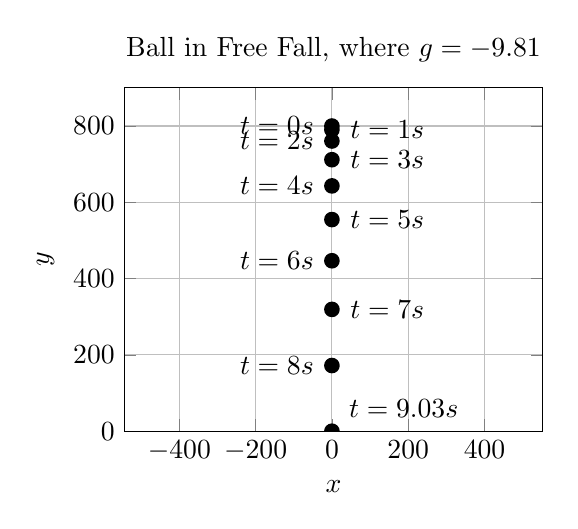
\begin{tikzpicture}
    \begin{axis}[
        title={Ball in Free Fall, where $g=-9.81$},
        axis equal,
        xlabel={$x$},
        ylabel={$y$},
        grid=major,
        legend pos=north west,
        width=\textwidth / 1.76,
        xmin=0, xmax=8,
        ymin=0, ymax=900,
        legend style={nodes={scale=1, transform shape}}, 
        ]
        % Vector from origin to (1/sqrt(2), 1/sqrt(2))
        \node[label={180:{$t=0s$}},circle,fill,inner sep=2pt] at (axis cs:0,800) {};
        \node[label={[label distance=0.01em]0:{$t=1s$}},circle,fill,inner sep=2pt] at (axis cs:0,790.19) {};
        \node[label={180:{$t=2s$}},circle,fill,inner sep=2pt] at (axis cs:0,760.76) {};
        \node[label={[label distance=0.01em]0:{$t=3s$}},circle,fill,inner sep=2pt] at (axis cs:0,711.71) {};
        \node[label={180:{$t=4s$}},circle,fill,inner sep=2pt] at (axis cs:0,643.04) {};
        \node[label={[label distance=0.01em]0:{$t=5s$}},circle,fill,inner sep=2pt] at (axis cs:0,554.75) {};
        \node[label={180:{$t=6s$}},circle,fill,inner sep=2pt] at (axis cs:0,446.84) {};
        \node[label={[label distance=0.01em]0:{$t=7s$}},circle,fill,inner sep=2pt] at (axis cs:0,319.31) {};
        \node[label={180:{$t=8s$}},circle,fill,inner sep=2pt] at (axis cs:0,172.16) {};
        \node[label={[label distance=0.01em]30:{$t=9.03s$}},circle,fill,inner sep=2pt] at (axis cs:0,0) {};
    \end{axis}
\end{tikzpicture}
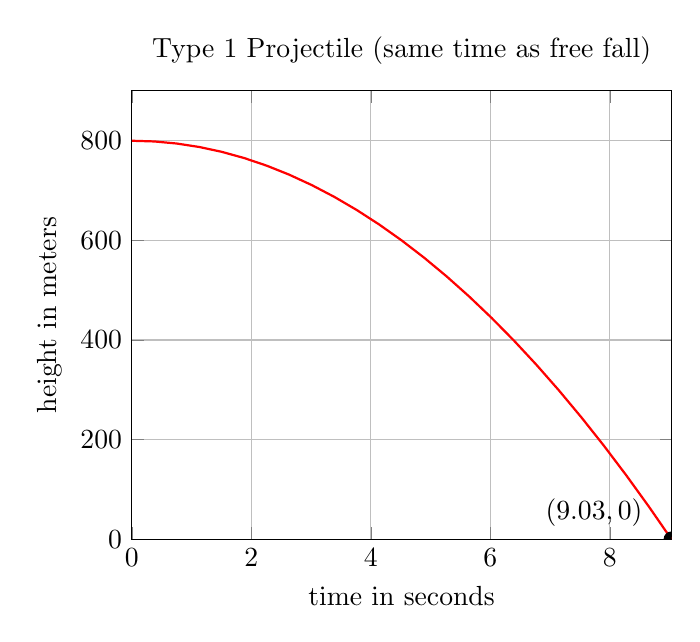
\begin{tikzpicture}
    \begin{axis}[
        title={Type 1 Projectile (same time as free fall)},
        xlabel={time in seconds},
        ylabel={height in meters},
        grid=major,
        domain=0:9.03,
        legend pos=north west,
        xmin=0, xmax=9.03,
        ymin=0, ymax=900,
        legend style={nodes={scale=1, transform shape}}, 
        ]
        % Vector from origin to (1/sqrt(2), 1/sqrt(2))
        \addplot [
            thick,
            red,
        ] ({x}, {800 - 9.81*x^2});
        \node[label={[label distance=0.4em]170:{$(9.03, 0)$}},circle,fill,inner sep=2pt] at (axis cs:9.03,0) {};
    \end{axis}
\end{tikzpicture}

\noindent Example Type 2 Projectile\\
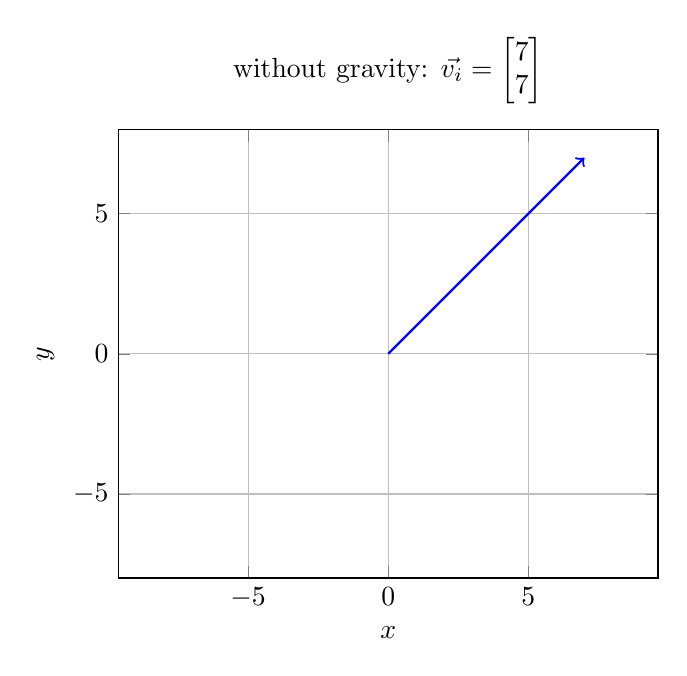
\begin{tikzpicture}
    \begin{axis}[
        title={without gravity: $\vec{v_i}=\begin{bmatrix}7\\7\end{bmatrix}$},
        axis equal,
        xlabel={$x$},
        ylabel={$y$},
        grid=major,
        legend pos=north west,
        xmin=-8, xmax=8,
        ymin=-8, ymax=8,
        legend style={nodes={scale=1, transform shape}}, 
        ]
        % Vector from origin to (1/sqrt(2), 1/sqrt(2))
        \addplot[->, thick, blue] coordinates {(0,0) (7, 7)};
    \end{axis}
\end{tikzpicture}
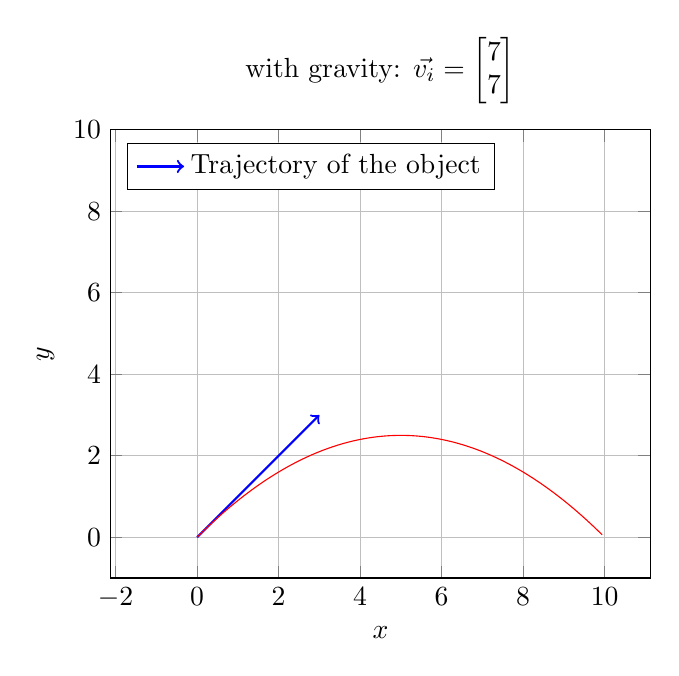
\begin{tikzpicture}
    \begin{axis}[
        title={with gravity: $\vec{v_i}=\begin{bmatrix}7\\7\end{bmatrix}$},
        axis equal,
        xlabel={$x$},
        ylabel={$y$},
        grid=major,
        samples=400,
        legend pos=north west,
        xmin=-1, xmax=10,
        ymin=-1, ymax=10,
        legend style={nodes={scale=1, transform shape}}, 
        ]
        % Vector from origin to (1/sqrt(2), 1/sqrt(2))
        \addplot[->, thick, blue] coordinates {(0,0) (3, 3)};
        \addplot [
            thin,
            red,
            domain=0:1.42,
            samples=100,
        ] ({7*x}, {7*x - 4.9*x^2});
        \addlegendentry{Trajectory of the object}

    \end{axis}
\end{tikzpicture}
\newpage

\noindent\section{Example Horizontal Problems}

\noindent 1) A car accelerates from rest at a constant rate of 5 m/s\(^2\) for 8 seconds. Calculate the final velocity and the displacement of the car.
\\ \hrule

\setlength{\columnsep}{1cm}
\setlength{\columnseprule}{0.2pt}
\begin{multicols}{3}
    \noindent
    \begin{flalign*}
        v_i &= 0 \, \text{m/s} & \\
        a &= 5 \, \text{m/s}^2 & \\
        t &= 8 \, \text{s} & \\
        v_f &= ? & \\
        s &= ?
    \end{flalign*}
    
    \noindent Using \( v_f = v_i + at \):
    \begin{flalign*}
        v_f &= 0 + (5)(8) \\
        v_f &= 40 \, \text{m/s}
    \end{flalign*}
    
    \noindent Using \( s = v_i t + \frac{1}{2} a t^2 \):
    \begin{flalign*}
        s &= (0)(8) + \frac{1}{2} (5)(8^2) \\
        s &= 0 + \frac{1}{2} (5)(64) \\
        s &= 160 \, \text{m}
    \end{flalign*}
\end{multicols}
\hrule

\noindent 2) A car accelerates from rest at $1.0$ $m/s^2$ for 20 s along a straight road. It then moves at a constant speed for half an hour. It then slows down uniformly to a stop in 30 s. Find the total distance covered by the car.\\ \hrule

\includegraphics[width=\textwidth]{Graphs/ABC Graph.png}\\

\hrule

\setlength{\columnsep}{1cm}
\setlength{\columnseprule}{0.2pt}
\begin{multicols}{3}
    \noindent\centering Segment A:
    \begin{flalign*}
        s_a &= \frac{1}{2} (v_f + v_i) t \\
        s_a &= \cancel{\frac{1}{2}} (\cancel{2}0)20 \\
        s_a &= 200m
    \end{flalign*}
    
    \noindent\centering Segment B:
    \begin{flalign*}
        &30min = (30 \times 60)s\\
        &v = 30 * 60 = 1800\\
        &1800s \times 20 m/s = 36000m\\
        &s_b = 36000m
    \end{flalign*}
    
    \noindent\centering Segment C:
    \begin{flalign*}
        &s_c = \frac{1}{2}(v_f + v_i)t\\
        &s_c = \cancel{\frac{1}{2}} (\cancel{2}0)30\\
        &s_c = 300m
    \end{flalign*}
\end{multicols}

\begin{center}{$s_{total} = \boxed{36500m}$}\end{center}
\newpage
\noindent\section{Vertical Problems}

\end{document}
